\section{Propuesta}

\small

\textbf{Research Website:} http://www.itorizaba.edu.mx

\textbf{Which libraries do you use or interested in using? (Select main one, but no more than 3):} CuDNN, NPP, OpenCV

\textbf{Research Domain/Field of Interest (Select main domain based on project but no more than 3):} Artificial Intelligence, Computer Vision and Machine Vision y Medical Imaging 

\textbf{Programming interfaces/language solutions used for GPU acceleration (Select no more than 3):} Anaconda, Python, Matlab

\textbf{Which Deep Learning Framework are you using (eg. TensorFlow, Torch, etc.):} Tensorflow, Keras, PyTorch

\textbf{Statement of Proposed Research: }

Cervical Cancer screening is a demanding procedure for the human expert. Their
training is done using a Data Base that serves as the Gold Pattern for all
technicians and they are evaluated exhaustingly to achieve high levels of
certainty, also, the training ensures that the technician is capable to detect
even the most little anomaly within a Papanicolau test smear as viewed with a
microscope. As the job consists of meticulously screen each individual cell for
anomalies, it inflicts stress in the technician’s eye and in the long term it
can harm his or her vision permanently. Also, the volume of work increases as
the availability of the test becomes widespread within vulnerable populations.
[1] The technician only have to detect one single anomalous cell to tag the
samples as cancerous, the sample is next passed to the pathologist for correct
diagnostics. The need for a system that helps the technician in the screening
problem increases as the accumulation of unreviewed samples becomes critical,
this is because the technician can’t overwork his or her eyes (most technicians
overwork their eyes to meet the quotas).

The problem is simple, detecting one anomalous cell inside a pap smear test
using a stock microscope. Our solution involves a system to detect anomalous
cells and an embedded implementation of such system using a single-board
computer (of low cost). 

Cell detection is going to be done with Deep Learning techniques as previous
work with other Artificial Intelligence techniques have been fructiferous. Our
research showed that Deep Learning is achieving high certainty and reliability
in fields such as Computer Vision, Image Classification and, important for this
project, Object Detection and its use in Medical Image Processing and
Computer-Aided Diagnosis is state-of-the-art. [2]

This project is going to serve as a starting point to teach and train
researchers in novel artificial intelligence algorithms and frameworks to tackle
Industrial Engineering problems not only within IMSS but in industries also. 

As the principal problem of developing and deploying Deep Learning models is the
amount of data available to build a particular model, our partnership with the
Mexican Social Security Institute is invaluable. They not only will provide the
same Golden Pattern database in which experts are trained, but are also will
provide medical experts and manpower to collect and improve such database with
field taken samples that will resemble the exact conditions on which the
detection device is going to be used. Tailored Digital Image Processing
algorithms are going to be applied to help the DL model by reducing variations
and improving contrast, lighting and hue for better detection, GPU will help us
to quickly test several of them and pick the best one. 

We aim to build a reliable database for training and testing different DL
models: Convolutional Neural Networks, Fully Convolutional Networks, Capsule
Networks and research for multi-input models that will include an image model
and another one (like LSTM for medical record analysis) for diagnosis and not
only for screening. Also, as our faculty members have expertise using
optimization techniques like Evolutionary Algorithms, Particle Swarm, Ant
Colony, Monte Carlo and we will use them in hyper-parameter optimization tasks
which are suited for GPU acceleration.

There exists a zoo of Deep Neural Networks architectures that are suited for a
specific or a broad spectrum of problems. Given that, we are going to test
several of these architectures: ResNet and its variants, VGG and its variants,
GoogleNet, AlexNet, RetinaNet, Yolo and its variants, etc. Training
methodologies are going to be as follow: Transfer Learning as a Feature
Extractor, Transfer Learning with Fine Tuning and, as we will get a large
database, training from scratch. We will try several datasets, and pre-trained
networks in this project. 

Sample variation are caused by different preparation and methods used to get a
Papanicolau Smear Test from a patient. Nurse skill and patient condition
decrease sample quality. Also, variation can come from the staining procedure,
as each nurse can prepare the sample with different concentrations of staining
chemicals. We will reduce this variation using DPI as proposed before and during
the Data Augmentation phase of DL training, modifying the image to simulate
different staining concentrations, blood presence and erasing known impurities. 

We want to get two models using this approach: the best overall model and the
best model that can be implemented in a single-board computer and provide real
life performance. Several of them will be tested, being Raspberry Pi the most
obvious candidate we will try other vendors and boards such as Asus Rock. The
cost of the final device is an important constraint so we will keep our choices
cheap as possible; Intel Movidious is also considered as it can boost the
performance of these cards in DL tasks.

We also aim to propose novel network architectures and test them against the
previous approach so we can get insight of how these models behave and
strengthen our knowledge in these new Artificial Intelligence Methodologies.
Capsule Networks are going to get special attention as they seem to manage
rotation and orientation more precisely, characteristics greatly present in cell
analysis [3].

We plan to use and apply the model generated by this project to improve research
in other areas in Medical Imaging and Computer-Aided Diagnosis, in particular,
cytological analysis, detection and classification. Traditional statistical
analysis and inference will be used to determine the best overall model, as we
plan to train and test several of them with the help of the GPU. 

Python language will be used to interface with C++ libraries that will power the
DPI algorithms and DL training. OpenCV has reliable Python bindings and we will
leverage this to implement the full application in the board’s LINUX Operative
System. Bindings to CuDNN are present in TensorFlow (TF) and PyTorch modules, we
will test both; Keras will be used for prototyping and a high level API for TF 

The final solution will be a device that, connected to a microscope, will assist
the expert in detecting anomalous cervical cells. Adapters are going to be 3d
printed to attach the camera to the microscope. The system has the benefit of a
screen to easily analyze the sample. The technician surveys the whole sample
looking for a single anomalous cell and the system will detect these cells and
provide insight in the form of a probability (using SoftMax). The expert will
only have to put the eye in the microscope when difficult or peculiar cases are
present, increasing efficiency and reducing eye stress.

As an overall goal, we are aiming to provide an improved Treatment Supply Chain,
leveraging our partnership with health organizations. We propose three more
steps after our screening solution:

\begin{itemize}
    \item{\textbf{Diagnostics:}} Our previous work using techniques such as
    Fuzzy Logic and traditional DPI for cancer screening serves as a foundation
    to achieve our overall goal. We can overcome our limitations in model
    complexity and computational power by using GPUs to accelerate Fuzzy Models
    and Fuzzy Image Segmentation; allowing us to create new and improve previous
    models with more rules for better inference power. [4] [5] Colposcopy image
    analysis using Deep Learning is also considered.
    \item{\textbf{Epidemiology:}} Medical data already gathered can be analyzed
    to provide epidemiological insight about cancer, high volumes of this data
    are available; we can evaluate risks in groups divided by age, income level,
    etc. Algorithms like K-Means (for segmentation) can be accelerated inside
    GPU allowing us to process patient data with effectiveness.
    \item{\textbf{Prevention:}} After identifying high risk populations, we can
    then take this insight and join it with regular patient data that is
    generated daily inside clinics (mostly Excel files). XG-Boost is the
    standard algorithm for processing tabular data and, as patient data is the
    most abundant kind of data inside the Treatment Supply Chain, we can make
    use of GPU acceleration to improve our boosting models.
\end{itemize}

1.	Jusman Y. Intelligent screening systems for cervical cancer. Scientific World Journal. 2014.

2.	Zheng Y. Review of Deep Learning Methods in Mammography, Cardiovascular, and Microscopy Image Analysis. Advances in Computer Vision and Pattern Recognition. 2017.

3.	Tajbakhsh N. On the Necessity of Fine-Tuned Convolutional Neural Networks for Medical Imaging. Advances in Computer Vision and Pattern Recognition. 2017.

4.	Gómez-Posada R. Development of an expert system as a diagnostic support of cervical cancer in atypical glandular cells, based on fuzzy logics and image interpretation. Computational and Mathematical Methods in Medicine. 2013.

5.	Y. Z. Parallel fuzzy connected image segmentation on GPU. Medical Physics. 2011.


\textbf{Equipment Requested:} GeForce

\textbf{Do you have or will you purchase a workstation or system to house the donated GPU?:} Yes

\textbf{Are you interested in sharing your work with the GPU community?:} Yes

\section{Correo de aceptación}

\begin{figure}[H]
    \centering
    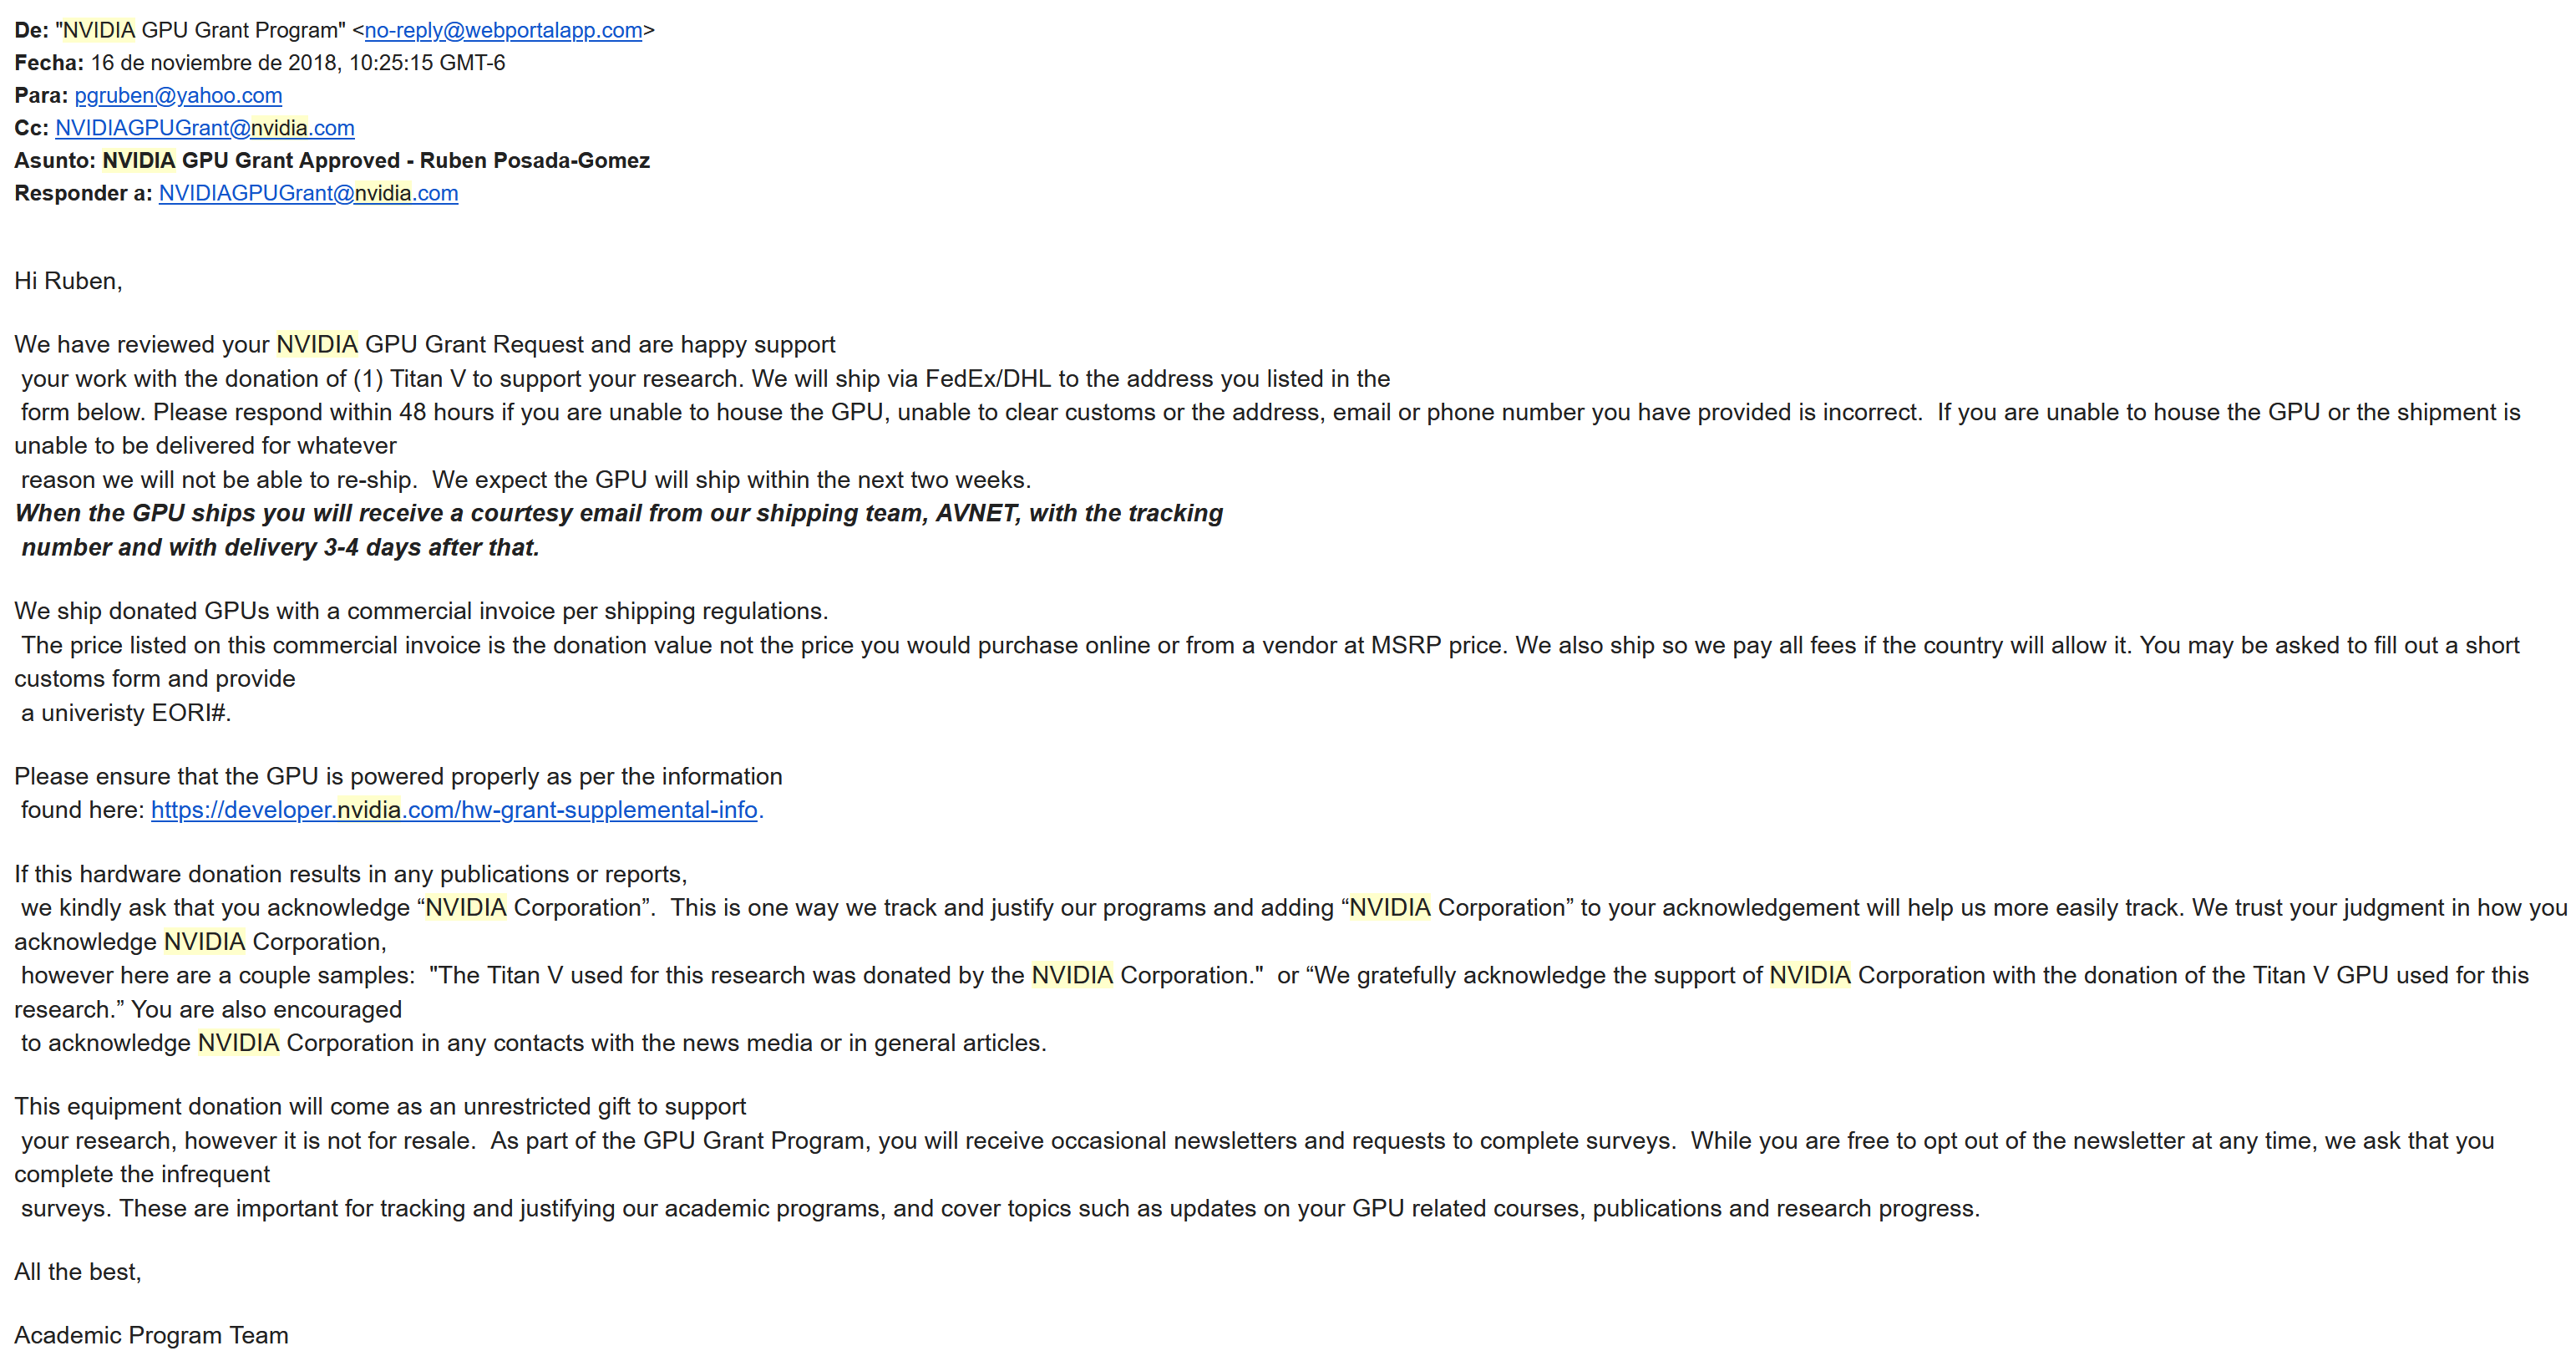
\includegraphics[width=\textwidth]{apendice_grant/correo_nvidia}
    \caption{Correo de aceptación para la donación}\label{fig:aceptaccion}
\end{figure}
